\section{Cactus Environment Big Step Semantics}

Of course, when compiling to machine code, we need a mechanical way to
efficiently implement the substitution and memoization as described in
call-by-need semantics. For this we turn to the recently developed Cactus
Environment $\mathcal{CE}$ Machine \cite{?}. We break the section in to two
parts. First, we describe environment representation, and the choice we make for
the $\mathcal{CE}$ machine. Next, we describe the big-step semantics of the
machine.

\subsection{Environment Representations}

As mentioned in Section~\ref{sec:back}, environments bind free variables to
closures. There is significant flexibility in how they can be represented. In
this section we review this design space in the context of existing work, both
for call by value and call by need.\footnote{Some work refers to this space as
\emph{closure} representation rather than \emph{environment}
representation~\cite{shao1994space,appel1988optimizing}.  Because the term
part of the closure is simply a code pointer and the interesting design
choices are in the environment, we refer to the topic as environment
representation.}

There are two common approaches to environment representation: \emph{flat}
environments and \emph{shared} environments (also known as linked
environments)~\cite{appel1988optimizing,shao1994space}. A flat environment is
one in which each closure has its own record of the terms its free variables are
bound to. A shared environment is one in which parts of that record can be
shared among multiple closures~\cite{appel1988optimizing,shao1994space}. For
example, consider the following term: $$(\lambda x.(\lambda y.t) (\lambda
z.t_1)) t_2$$ Assuming the term $t$ has both $x$ and $y$ as free variables, we
must evaluate it in the environment binding both $x$ and $y$.  Similarly,
assuming $t_1$ contains both $z$ and $x$ as free variables, we must evaluate it
in an environment containing bindings for both $x$ and $z$. Thus, we can
represent the closures for evaluating $t$ and $t_1$  as $$t[x=t_2[\bullet],
y=c]$$ and $$t_1[x=t_2[\bullet], z=c_1]$$ respectively.  These are examples of
\emph{flat} environments, where each closure comes with its own record of all of
its free variables. Because of the nested scope of the given term, $x$ is bound
to the same closure in the two environments. Thus, we can also create a shared,
linked environment, represented by the following diagram:

\begin{center}
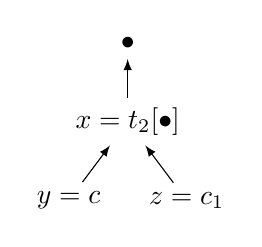
\begin{tikzpicture}[ 
  edge from parent path={(\tikzchildnode\tikzchildanchor) edge [-latex] (\tikzparentnode\tikzparentanchor)},
  level distance=1cm
]
\node (d) {$\bullet$} child{node (a) {$x=t_2[\bullet]$} child{node (b) {$y=c$}} child{node (c)
{$z=c_1$}}};

\end{tikzpicture}
\end{center}
Now each of the environments is represented by a linked list, with the binding
of $x$ shared between them. This is an example of a \emph{shared} environment
~\cite{appel1988optimizing}. This shared, linked structure dates back to the 
first machine for evaluating expressions: Landin's SECD
machine~\cite{landin1964mechanical}.

The drawbacks and advantages of each approach are well known. With a flat
environment, variable lookup can be performed with a simple offset
~\cite{jonesstg,appel2006compiling}. On the other hand, significant
duplication can occur, as we will discuss in Section~\ref{sec:exist}.
With a shared environment, that duplication is removed, but at the cost of
possible link traversal upon dereference. 

As with most topics in compilers and abstract machines, the design space is
actually more complex. For example, Appel and Jim show a wide range of hybrids
~\cite{appel1988optimizing} between the two, and Appel and Shao
~\cite{shao1994space} show an optimized hybrid that aims to achieve the benefits
of both approaches. And as shown in the next section, choice of evaluation
strategy further complicates the picture.

\subsection{Existing Call-by-Need Environments} \label{sec:exist}

Existing call by need machines use flat environments with a heap of
closures~\cite{jonesstg,TIM,johnsson1984efficient,boquist1997grin}. These
environments may contain some combination of primitive values and pointers into the
heap ($p$ below). The pointers and heap implement the memoization of results
required for call by need. Returning to the earlier example, $(\lambda
x.(\lambda y.t) (\lambda z.t_1)) t_2$, we can view a simplified execution state
for this approach when entering $t$ as follows:

\begin{center}
\textbf{Closure}
\begin{align*}
t[x=p, y=p_1] \\
\end{align*}
\textbf{Heap}
\begin{align*}
p &\mapsto t_2[\bullet] \\
p_1 &\mapsto \lambda z.t_1[x=p] 
\end{align*}
\end{center}

If $t_2[\bullet]$ is not in WHNF (this sort of unevaluated closure is called a
\emph{thunk}~\cite{ingerman1961way,peyton1992implementing}), then if it is
entered in either the evaluation of $t$ or $t_1$, the resulting value will
overwrite the closure at $p$. The result of the computation is then shared with
all other instances of $x$ in $t$ and $t_1$. In the case that terms have a large
number of shared variables, environment duplication can be expensive.
Compile-time transformation ~\cite{peyton1992implementing} (tupling arguments)
helps, but we show that the machine can avoid duplication completely.

Depending on $g$, either or both of the closures created for its arguments may
not be evaluated.  Therefore, it is possible that the work of creating the
environment for that thunk will be wasted. This waste is well known, and
existing approaches address it by avoiding thunks as much as possible
~\cite{jonesstg,johnsson1984efficient}. Unfortunately, in cases like the above
example, thunks are necessary. Indeed, even if we tuple the closures for $x$,
$y$, and $z$, that tuple could be wasted if neither $t$ nor $t'$ is used. Thus,
we would like to minimize the cost of creating such thunks.

Thunks are special in another way.  Recall that one advantage of the flat
environments is quick variable lookups. In a lazy language, this advantage is
reduced because \emph{a thunk can only be entered once}. After it is entered, it
is overwritten with a value, so the next time that heap location is entered it
is entered with a value and a different environment. Thus, the work to ensure
that the variable lookup is fast is used only once. This is in contrast to
a call by value language, in which every closure is constructed for a value,
and can be entered an arbitrary number of times. 

A more subtle drawback of the flat environment representation is that
environments can vary in size, and thus a value in WHNF can be too large to fit
in the space allocated for the thunk it is replacing. This problem is discussed
in~\cite{jonesstg}, where the proposed solution is to put the value closure in
a fresh location in the heap where there is sufficient room. The original
thunk location is then replaced with an indirection to the value at the freshly
allocated location. These indirections are removed during garbage collection,
but do impose some cost, both in runtime efficiency and implementation
complexity~\cite{jonesstg}.

We have thus far ignored a number of details with regard to current
implementations. For example, the STG machine can split the flat environment, so
that part is allocated on the stack and part on the heap.  The TIM allocates its
flat environments separately from its closures so that each closure is a code
pointer, environment pointer pair~\cite{TIM} while the STG machine keeps
environment and code co-located~\cite{jonesstg}. Still, the basic design
principle holds: a flat environment for each closure allows quick variable
indexing, but with an initial overhead.

To summarize, the flat environment representation in a call by need language is
whenever a term might be needed, the necessary environment is constructed from
the current environment.  This operation can be expensive, and it is wasted if
the variable is never entered. In this work, we aim to minimize this potentially
unnecessary overhead.

Figure~\ref{fig:designspace} depicts the design space relevant to this paper.
There are existing call by value machines with both flat and shared
environments, and call by need machines with flat environments. As far as we are
aware, we are the first to use a shared environment to implement lazy
evaluation.

\begin{figure*}
\begin{tabularx}{\textwidth}{l | X | X}
                & Flat Environment     & Shared Environment \\ \hline
  Call by need  & STG~\cite{jonesstg}, 
                  TIM~\cite{TIM}, 
                  GRIN~\cite{boquist1997grin} 
                & $\mathcal{CE}$ Machine (this paper) \\
  Call by value & ZAM~\cite{leroy1990zinc}, 
                  SML/NJ~\cite{appel1991standard}
                & ZAM,
                  SECD~\cite{landin1964mechanical}, 
                  SML/NJ \\
\end{tabularx}
\caption{Evaluation strategy and environment structure design space. Each
acronym refers to an existing implementation. Some implementations use multiple
environment representations.}
\label{fig:designspace}
\end{figure*}

\subsection{Big Step Semantics}

Our big step semantics closely resemble the standard call-by-need semantics,
with a few changes for one purpose: instead of standard lambda terms, we now are
using terms with deBruijn indices, and closing the the lambda term under a
pointer into a shared environment structure.  

The big step semantics can be seen in Figure~\ref{fig:bigstepcem}. The
\texttt{clu} function is a partial function that looks up a closure in the
shared environment. Here we use a direct function, but later this will be
replaced by a relation, as it will clearly take a non-constant number of
instructions to execute. Our abstraction rule is identical to the call-by-name
case, and the application rule evaluates the left hand side, then binds the
argument closure to a fresh location in the heap, which extends the environment
of the function computed on the left hand side. Then if the body with this
extended environment evaluates to a value, then the application as a whole
evaluates to a value.

We define a cactus environment machine state to be well formed if, like the
call-by-name semantics, a closure bound in the heap is closed to the left.
We also require the closure in question to be closed under the reachable heap,
and all domain variables to be unique across both the unreachable and reachables
heaps. Because we are using deBruijn indices, when referring to a fresh heap
location, we don't require freshness with respect to a substitution term,
because there is no substitution. This will be important when relating the two
states. We have the following lemma showing that well-formedness is preserved
through evaluation: 

\begin{lstlisting}
Lemma well_formed_step : ∀ c v, well_formed c → c ⇓ v → well_formed v.
\end{lstlisting}

This proof proceeds by induction on the step relation. For the \texttt{Id} rule,
it follows from the fact that the current closure is closed under the reachable
heap, so that we may safely insert it into a location in the unreachable heap
while retaining that it stays closed under the heap to the left. In addition, we
can take a closure from somewhere in the reachable heap, and safely shift our
reachable heap over to the left of that closure while making that closure our
current closure, corresponding to entering a closure. Note that because we
inform.     

\begin{figure}
\begin{lstlisting}
Inductive step : configuration → configuration → Prop :=
  | Id : ∀ M B x y z Φ Φ' Υ Ψ v e, clu v z (Υ ++ x↦cl M y::Φ) = Some (x, M) → 
      ⟨Φ & x↦cl M y, Υ, Ψ⟩M ⇓ ⟨Φ' & x↦cl M y, Υ, Ψ⟩close (:λB) e →
    ⟨Φ, x↦cl M y, Υ & Ψ⟩close v z ⇓ ⟨Φ', x↦ cl (close (:λB) e) y, Υ & Ψ⟩close (:λB) e
  | Abs : ∀ N Φ Ψ e, ⟨Φ & Ψ⟩close (:λN) e ⇓ ⟨Φ & Ψ⟩close (:λN) e
  | App : ∀ N M B B' Φ Φ' Ψ Υ f e ne ae, 
                  f ∉ domain (Ψ ++ Φ') → 
          ⟨Φ & Ψ⟩close M e ⇓ ⟨Φ' & Ψ⟩close (:λB) ne → 
      ⟨Φ', f ↦cl (close N e) ne & Ψ⟩close B f ⇓ ⟨Υ & Ψ⟩close (:λB') ae   →
              ⟨Φ & Ψ⟩close (M@N) e ⇓ ⟨Υ & Ψ⟩close (:λB') ae
where " c1 '⇓' c2 " := (step c1 c2).
\end{lstlisting}
\caption{Big Step Semantics for $\mathcal{CE}$}
\label{fig:bigstepcem}
\end{figure}

\subsection{Bisimulation with Call-by-Need}

Intuitively, to define our bisimulation relation between the call-by-need
semantics and the $\mathcal{CE}$ semantics, we need to relate how heap locations
are dereferenced. In the call-by-need semantics, when we bind a variable to a
closure, we append a fresh heap location and substitute all instances of that
variable with said heap location. In contrast, our $\mathcal{CE}$ machine
extends its shared environment with an indirection, creating a fresh heap
location that points to the previous environment, which ensures that all
variables of deBruijn index 0 will point to the correct closure in the heap,
while all other deBruijn indices will be incremented to point to their correct
closures. In other words, we have two different mechanisms to reach a term, or
closure, 

Our bisimulation relation between call-by-need and the big step cactus
environment semantics requires a few different properties. First, we require
that both states are well formed. Second, we need a way to relate heap
locations. Because our freshness conditions are different for the two semantics,
we cannot, without loss of generality, choose a freshness function that operates
on heap domains and use equality for our heap domain relation. Instead, we must
generate and retain an isomorphism between $\mathcal{CE}$ and CBN heap
locations. Thirdly, we need a way to relate terms with free variables from
deBruijn indices to standard indices. For this, we use an logical relation that
corresponds to a type of \emph{locally nameless} representation \cite{?}.
Indeed, one can show that the relation holds iff the two terms can be translated
into equal locally nameless terms, modulo the free variables being related by
the heap location isomorphism.  See the \texttt{eq\_terms} for the definition of
this relation.

\begin{figure}
\begin{lstlisting}
Inductive eq_terms_rel (m:list nat) (env:nat) (h:cem.heap) iso : expr.tm → db.tm → Prop :=
  | eq_lvar : ∀ v v', indexofn v m = Some v' → 
                  eq_terms_rel m env h iso (expr.var v) (db.var v')
  | eq_gvar : ∀ v x v' cl,     x >= length m → 
                       cem.clu (x - length m) env h = Some (v',cl) →
                              In (v, v') iso →
                  eq_terms_rel m env h iso (expr.var v) (db.var x)
  | eq_abs : ∀ v b b', eq_terms_rel (v::m) env h iso b b' → 
                  eq_terms_rel m env h iso (expr.abs v b) (db.lam b')  
  | eq_app : ∀ l l' n n', eq_terms_rel m env h iso l l' → eq_terms_rel m env h iso n n' → 
                            eq_terms_rel m env h iso (expr.app l n) (db.app l' n')
.

Definition eq_terms (t:expr.tm) (c:cem.closure) (h:cem.heap) iso : Prop := match c with
    cem.close e env => eq_terms_rel [] env h iso t e end.
\end{lstlisting}
\caption{Relation for equivalent terms. Terms are equivalent if they are
translated into equivalent related terms. }
\label{fig:eqterms}
\end{figure}

For relating the heaps of call-by-need and $\mathcal{CE}$, we check that each
location is isomorphic, and that each term-closure pair is equivalent under
the heaps and the isomorphism.  

\begin{figure}
\begin{lstlisting}
Inductive related_lists {a b} (r : a → b → list a → list b → Prop) : list a → list b → Prop :=
  | rel_nil : related_lists r nil nil
  | rel_cons : ∀ x xs y ys, 
      r x y xs ys → 
      related_lists r xs ys → 
      related_lists r (x::xs) (y::ys).

Definition eq_heaps (h : cem.heap) (h' : cbn.heap) iso := 
  related_lists (λ x y tl _, match x,y,tl with
  | (l, cem.cl c e), (l', t), tl => In (l, l') iso ∧ eq_terms t c tl iso
  end) h h'.
\end{lstlisting}
\caption{Relation for relating heaps of call-by-need and $\mathcal{CE}$}
\label{fig:eqheaps}
\end{figure}

Finally, we can combine the two notions of equivalence into our bisimulation
relation. We require that the current terms are equivalent as well as the heaps.
Note that we require the concatenation of the unreachable and reachable heaps to
be equivalent, as well as the reachable heaps in isolation. It would be
sufficient to show that the reachable heaps have equivalent size, but having
this stronger definition allows for easier proof management. 

\begin{figure}
\begin{lstlisting}
Definition eq_confs (c: cem.configuration) (c':cbn.configuration) iso : Prop := 
  cem.well_formed c ∧ cbn.well_formed c' ∧ 
  match c, c' with
  | cem.conf h ur cl, cbn.st h' ur' e' => eq_terms e' (cem.st_clos c) (cem.reachable c) iso
                                        ∧ eq_heaps (ur ++ h) (ur' ++ h') iso
                                        ∧ eq_heaps h h' iso
  end.
\end{lstlisting}
\caption{Relation for equivalent configurations for call-by-need and
$\mathcal{CE}$.}
\label{fig:eqconfs}
\end{figure}

For our proof that the relation is indeed a bisimulation,
\texttt{cbn\_cem\_bisim}, we proceed by induction on each of the step relations.
For the \texttt{Id} rules for each semantics, the proof follows from the fact
that we retain that each respective lookup function for a given related
term/closure looks up an isomorphic location, and therefore an equivalent
term/closure. This step of the rule requires the reachability conditions that
we've painstakingly managed. Without reachability constraints, we wouldn't be
able to ensure that upon updating a value the location has retained its original
closure or term. In other words, we've implicitly ensured that the heaps are
acyclic. 

The abstraction rules are trivial, but the \texttt{App} rules are again fairly
challenging. We must prove that if either machine takes an application step, all
of the equivalences are preserved through extending the environment and adding
fresh heap locations. Note that this is the primary reason for using the
inductive relation for the term equivalence: a first attempt was to use a direct
computational approach. One can declare terms equal iff they compile to
equivalent (modulo heap isomorphism) locally nameless terms. The relational
approach is equivalent to this computational approach, but allows for better
inductive reasoning. 

